\documentclass{article}
\title{Diagonal projections and rank histograms for measuring the distance between estimated copulas and observed data}
\author{Ma\"{e}l Forcier}
\date{May 2017}

\usepackage[utf8]{inputenc}
\usepackage{mathtools}
\usepackage{amsfonts}
\usepackage{amsmath}
\usepackage{amsthm}
 \usepackage{relsize}
\usepackage{stmaryrd}
\usepackage{dsfont} 
\renewcommand\qedsymbol{$\blacksquare$}

\begin{document}
   \maketitle
   \section{Introduction}
  	To create scenarios for renewable energies production, we need to be able to measure the dependance through space and time or between different sources. To focus on the correlation, we use copulas. Giving a set of datas, different methods exist to choose the best copulas and parameters that will best fit and model our datas. Nevertheless, we need tools to verify and measure how each of the copulas fit our observed data. Moreover, we need a tool that focus on the tails where the dependance matters a lot for us. I will briefly present in section 1, the loglikelihood which is a classical way to measure the overall fit of a distribution. Then, I will describe more precisely a way to measure how a copula fit the datas in the tail using rank histogram on diagonal projections.
  	
   \section{Loglikelihood}
   Present briefly the loglikelihood. Refer to a good paper explaining loglikelihood ?
   
   
   \section{Solving the problem of unreproducibility}
	Each day j, we look at a set of data including for example a description of the state of the system early in the morning and the observations of the 90 previous days. With this set of data, we are able to choose a distribution represented by its cumulative density function \begin{math}F_j\end{math} with a set of parameters \begin{math} \theta_j \end{math} that we hope will predict the best what will happen on day j. Some techniques are presented in \cite{vineconstruction} or \cite{fourcopulas} but we will not focus on them in this article. We now want to verify if this distribution was well chosen. \newline
	\newline
   Unfortunately, we only observe what happens on the day j once. Let us note \begin{math}O_j \end{math} the day j observation. \begin{math}O_j \end{math} is not sufficient to check if this random variable follow the distribution \begin{math} F_j \end{math}. Moreover, each day is different and for instance another day \begin{math}i\neq j\end{math}  will give a different distribution \begin{math} F_i \end{math} with different parameters \begin{math} \theta_i \end{math}. Thus, it is impossible to verify if each distribution is correct each day. Nevertheless, their are techniques to verify if our procedure is valid and if the estimation of distributions makes sense. \newline
   \newline
   
   Let us define \begin{math}U_j = F_{j}(O_{j})\end{math}. It is easy to prove that \begin{math} U_j\end{math} should have a uniform distribution. (This classical result is often used to generate a random variable X following cumulative density function F with uniform random variable U : \begin{math}X = F^{-1}(X)\end{math}.)
   As all \begin{math}U_j\end{math} are computed independantly, all the \begin{math}U_j\end{math} must be independant and distributed uniformly.\newline
   \newline
   We now have a set of observation \begin{math} \textbf{U} = (U_1,..U_n)\end{math} that should be independant and uniformly distributed on [0,1]. We can now compute the extent to which it follows a uniform distribution for example by computing the Earth Mover Distance between the empirical distribution of U and the uniform distribution or by using rank histograms.
    
	\section{Rank histograms}   
   
   Imagine we have our problem in 1 dimension.
   Give an example in dimension 1.
   Present rank histograms refers to \cite{hamill2000}
   \newline
   \newline
   As one can see in \cite{hamill2000}, the biggest problem with rank histograms is that they are primarly useful only in one dimension. So we have to make projection. Projecting on the marginals is useless because what we care about is the dependance. Thus, we will project on the diagonals. This way we can measure the fit of the copulas in the corner that we are interested in.
   
   
	\section{Earth Mover Distance}
	 \newtheorem{definition}{Definition}
	 \begin{definition}
	 The \textbf{Earth Mover Distance} (EMD) between two histograms $P=((x_i,p_i))_i$ and $Q=((y_j,q_j))_j$ is :
	 \begin{equation*}	 
	 EMD(P,Q) = \frac{\min\limits_{(f_{i,j}) \in F} \sum_{i,j} f_{i,j} d_{i,j}}{ \min(\sum_i p_i, \sum_i q_i)}
	 \end{equation*}
	 \newline
	 where \begin{math}F=\{(f_{i,j})| f_{i,j}\geq 0,\sum\limits_{i} f_{i,j} \leq P_i, \sum\limits_{j} f_{i,j} \leq Q_j, \sum\limits_{i,j} f_{i,j} = \min(\sum\limits_i p_i, \sum\limits_i q_i)\} \end{math}\newline
	 and $d_{i,j}$ is the distance between $x_i$ and $y_j$.
	\end{definition}
	
	In our problem, we look at histograms of distribution with real density function. So, with probability 1 we will not have the same result twice. Thus, the weight of our histograms will just be 1 for each value : $\forall i, q_i =1, \forall j, p_j=1$.\newline
	Moreover, we will only consider vectors with same dimension n. We can now simplify the notation and define the EMD between two vectors :
	
	
	\begin{definition}
	 The \textbf{Earth Mover Distance} (EMD) between two vectors $\textbf{u}=(u_1,...,u_n)$ and $\textbf{v}=(v_1,...,v_n)$ of dimension n is :
	 \begin{equation*}
	 EMD(\textbf{u},\textbf{v}) = \frac{1}{n}\min\limits_{(f_{i,j}) \in F} \sum_{i=1}^n \sum_{j=1}^n f_{i,j} d_{i,j}
	 \end{equation*}
	 \newline
	 where \begin{math}F=\{(f_{i,j})| f_{i,j}\geq 0,\sum\limits_{i=1}^n f_{i,j} \leq 1, \sum\limits_{j=1}^n f_{i,j} \leq 1, \sum\limits_{i=1}^n \sum\limits_{j=1}^n f_{i,j} = n\}\end{math}
	 \newline
	 and $d_{i,j}=|u_i-v_j|$
	\end{definition}
	
	Solving this linear program is possible but there is a faster way to compute the EMD thanks to the following property : 
	
	\newtheorem{property}{Property}
	\begin{property}
	For any vectors \textbf{u} and \textbf{v} of dimension n :
	\begin{equation*}	
	EMD(\textbf{u},\textbf{v}) = \frac{1}{n} \sum_{i=1}^n |\tilde{u}_i - \tilde{v}_i| =  \frac{1}{n}||\tilde{\textbf{u}}-\tilde{\textbf{v}}||_1
	\end{equation*}
	where $\tilde{\textbf{x}}$ is the sorted vector of $\textbf{x}$ :
	\newline
	$\{x_1,...,x_n\}=\{\tilde{x}_1,...,\tilde{x}_n\}$ and $\forall i \leq j, \tilde{x}_i \leq \tilde{x}_j$\newline
	\end{property}



	\textbf{Demonstration :}\newline
	\newline
	First we have :
	\begin{multline*}
	\begin{split}
	F	&= \{(f_{i,j})| f_{i,j}\geq 0,\sum\limits_{i=1}^n f_{i,j} \leq 1, \sum\limits_{j=1}^n f_{i,j} \leq 1, \sum\limits_{i=1}^n \sum\limits_{j=1}^n f_{i,j} = n\} \newline \\
		&= \{(f_{i,j})| f_{i,j}\geq 0,\sum\limits_{i=1}^n f_{i,j} = 1, \sum\limits_{j=1}^n f_{i,j} = 1 \}
	\end{split}
	\end{multline*}
	The way $\supset$ is trivial.\newline
	\newline
	Let be $(f_{i,j})_{i,j} \in F$ and let us suppose that $\exists i_0, \sum\limits_{i=1}^n f_{i_0,j} < 1 : \sum\limits_{i=1}^n f_{i_0,j} = 1-\epsilon $.\newline
	Thus, $\sum\limits_{i=1}^n \sum\limits_{j=1}^n f_{i,j} \leq 1-\epsilon +\sum\limits_{i=1,i\neq i_0}^n 1= n-\epsilon < n $\newline
	$(f_{i,j})_{i,j} \notin F$ : Contradiction \newline
	\newline
	We will now demonstrate that it exists $f_{i,j}$ integers that solve the minimum problem. This a classical demonstration using several theorems. For any precision, see the chapter 2 of \cite{gaubert}.\newline
	
	Let us define $M = (M_{k,(i,j)}) \in \mathcal{M}_{2n,n^2}(\mathbb{R})$ with :\newline
	\[
   		M_{k,(i,j)} =  \begin{cases}
        1  & \quad \text{if } k=i \\
    	-1 & \quad \text{if } k=j+n\\
    	0 & \quad \text{else}\\
  	\end{cases}
  	\]
	Because $1\leq i,j \leq n$ the cases are incompatible.\newline
	\newline
	We now have :\newline
	\begin{equation*}
	F = \{(f_{i,j})| f_{i,j}\geq 0, Mf = B \}
	\end{equation*}
	where $B = 
 	\begin{pmatrix}
 	 1  \\
 	 \vdots \\
  	1 \\
  	-1 \\
  	\vdots  \\
  	-1 
 	\end{pmatrix}$\newline
 	\newline
 	The coefficient of M are just -1,0 and 1 and 
	M has just once 1 and once -1 on each of its column. \newline
	Thanks to the Poincaré lemma (see \cite{gaubert} chapter 2), we can say that M is totally unimodulary. Because B has integer coefficient, we can say that all extreme points of F have integer coefficients.\newline
	So, we finally have it exists $f_{i,j}$ integers that solve the minimization problem.\newline
	\newline
	Let $(f_{i,j})_{i,j}$ solve the mnimization problem with integer coefficients.\newline
	$\forall i, \forall j, 0\leq f_{i,j} \leq 1$ and $f_{i,j}\in \mathbb{N} \Rightarrow f_{i,j} =0$ or $ f_{i,j} =1$ \newline
	$\forall i, \sum\limits_{j=1}^n f_{i,j} = 1 \Rightarrow \exists ! j_0,  f_{i,j_0} =1$\newline
	$\forall j, \sum\limits_{i=1}^n f_{i,j} = 1 \Rightarrow \exists ! i_0,  f_{i_0,j} =1$\newline
	\newline
	We now have :
	\begin{equation*}
	\exists \sigma \in \mathfrak{S}_n, f_{i,j} =  \begin{cases}
        1  & \quad \text{if } j=\sigma(i) \\
    	0 & \quad \text{else}\\
  	\end{cases}
	\end{equation*}
	So,
	\begin{equation*}
	EMD(\mathbf{u},\mathbf{v}) = \min\limits_{\sigma \in \mathfrak{S}_n} \sum_{i=1}^n d_{i,\sigma{i}} = \min\limits_{\sigma \in \mathfrak{S}_n} \sum_{i=1}^n |u_i-v_{\sigma (i)}|
	\newline
	\newline
	\end{equation*}
	
	We now have to prove that this min is reached when $(u_i)_i$ is sorted in the same order than $(v_{\sigma (i)})_i$. Since the indexes have symetric roles and are just notations indicating coefficients, we can consider that u and v are sorted :\newline
  $\forall i \leq j, u_i \leq u_j, v_i \leq v_j$\newline
  With this notation, we need to prove that this minimum is reached for $\sigma = Id$.\newline
  \newline
  Suppose that $\sigma \neq Id$ reaches the minimum, so $supp(\sigma)\neq \emptyset$ and $supp \sigma$ contains at least two elements. Let us define:
 
  \begin{multline*}
	\begin{split}
	q	&=  \max supp(\sigma)\\
	p	&=  \sigma^{-1}(q) \\
	r 	&= \sigma (q)
	\end{split}
	\end{multline*}
	
	We have $q\leq p$ and $r\leq p$, so $u_q\leq u_p$ and $v_r\leq v_p$.
	
	
	\begin{itemize}
	\item Case 1 : $u_p \leq u_q \leq v_r \leq v_q$
	\end{itemize}
	
	\begin{multline*}
	\begin{split}
	|u_p-v_q| + |u_q-v_r|	&=  v_q-u_p+v_r-u_q\\
		&=  v_r-u_p+v_q-u_q \\
	 	&= |u_p-v_r|+|u_q-v_q|
	\end{split}
	\end{multline*}
		
	
	\begin{figure}
      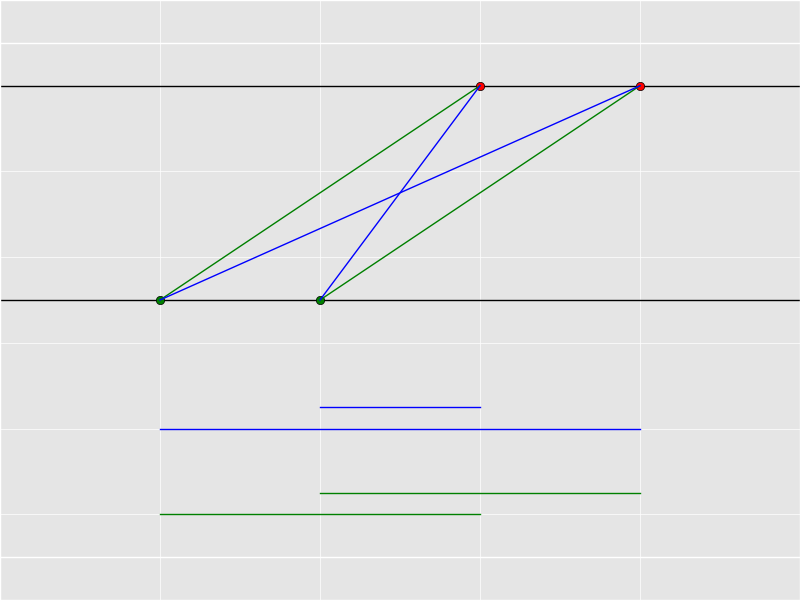
\includegraphics[width=0.5\textwidth]{demo_sort1.png}
    \caption{Graphic representation of case 1 : \emph{The upper black line represents \textbf{v} and the lower one \textbf{u}. The red points are from left to right $v_r$ and $v_q$ and The green points are from left to right $u_p$ and $u_q$. The blue lines represent what the cost when using $\sigma$ and the green lines  the cost when using $\tilde{\sigma}$. } }
\end{figure}

\begin{itemize}
	\item Case 2 : $u_p\leq v_r \leq u_q \leq v_q$
	\end{itemize}
	
	\begin{multline*}
	\begin{split}
	|u_p-v_q| + |u_q-v_r|	&\leq  |u_p-v_q|\\
		&=  v_q-u_p \\
	 	&= v_q-u_q+u_q-u_p\\
	 	&\leq v_q-u_q+v_r-u_p\\
	 	&= |u_q-v_q|+|u_p-v_r|
	\end{split}
	\end{multline*}

\begin{figure}
  
    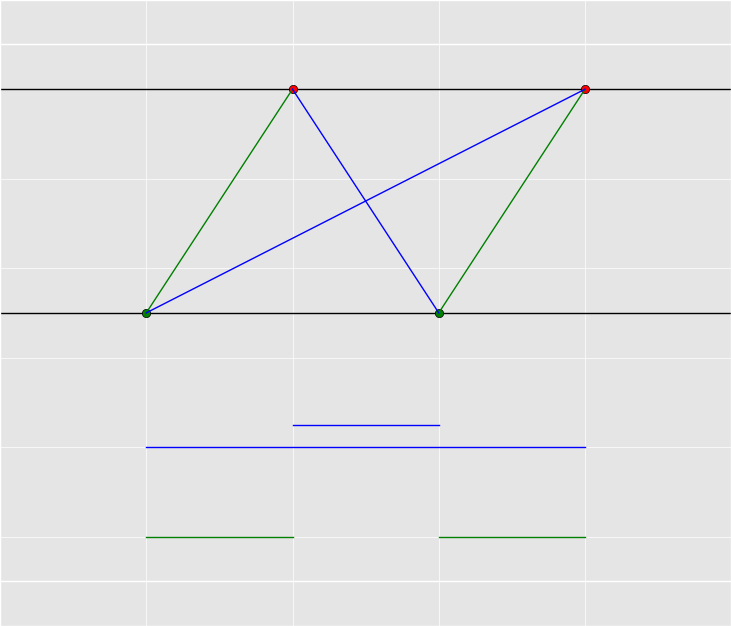
\includegraphics[width=0.5\textwidth]{demo_sort2.png}
     \caption{Graphic representation of case 2 : \emph{The upper black line represents \textbf{v} and the lower one \textbf{u}. The red points are from left to right $v_r$ and $v_q$ and The green points are from left to right $u_p$ and $u_q$. The blue lines represent what the cost when using $\sigma$ and the green lines  the cost when using $\tilde{\sigma}$. } }
\end{figure}

\begin{itemize}
	\item Case 3 : $u_p\leq v_r \leq v_q \leq u_q$
	\end{itemize}
	
\begin{figure}
  
    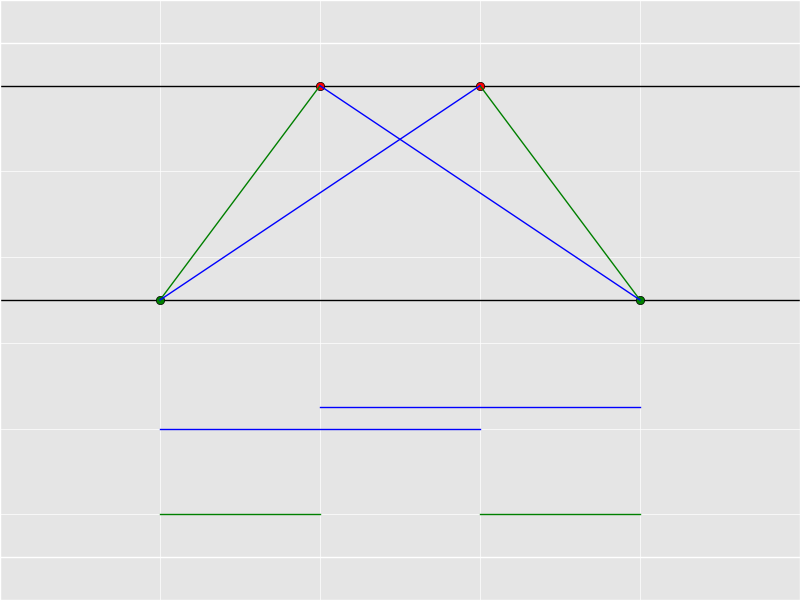
\includegraphics[width=0.5\textwidth]{demo_sort3.png}
     \caption{Graphic representation of case 3 : \emph{The upper black line represents \textbf{v} and the lower one \textbf{u}. The red points are from left to right $v_r$ and $v_q$ and The green points are from left to right $u_p$ and $u_q$. The blue lines represent what the cost when using $\sigma$ and the green lines  the cost when using $\tilde{\sigma}$. } }
\end{figure}	
	
	\begin{multline*}
	\begin{split}
	|u_p-v_q| + |u_q-v_r|	&=  v_q-u_p+u_q-v_r\\
		&=  u_q-u_p+v_q-v_r \\
	 	&\leq u_q-u_p\\
	 	&= u_q-v_q+v_q-u_p\\
	 	&\leq u_q-v_q+v_r-u_p\\
	 	&= |u_q-v_q|+|u_p-v_r|
	\end{split}
	\end{multline*}
	
	
	\begin{itemize}
	\item Case 4 : $v_r\leq v_q \leq u_p \leq u_q$\newline
	Same as case 1 by inversing the symetric roles of \textbf{u} and \textbf{v}.
	
	\item Case 5 : $v_r\leq u_p \leq v_q \leq u_q$\newline
	Same as case 2 by inversing the symetric roles of \textbf{u} and \textbf{v}.
	
	\item Case 6 : $v_r\leq u_p \leq u_q \leq v_q$\newline
	Same as case 3 by inversing the symetric roles of \textbf{u} and \textbf{v}.
	\end{itemize}

In all this cases, we have :
\begin{equation*}
	|u_p-v_q| + |u_q-v_r| \leq |u_q-v_q|+|u_p-v_r|
\end{equation*}
Let us define $\tilde{\sigma} = \sigma \circ (p q)$ :\newline
\begin{equation*}
 	\forall i \notin \{p,q\}, \tilde{\sigma} (i)=\sigma (i)
\end{equation*}
\begin{equation*}
 	\tilde{\sigma} (p)=r
\end{equation*}
\begin{equation*}
 	\tilde{\sigma} (q)=q
\end{equation*}

Then  we have

\begin{multline*}
	\begin{split}
	\sum_{i=1}^n |u_i-v_{\sigma (i)}|	&= \sum_{i\notin \{p,q\}} |u_i-v_{\sigma (i)}|+|u_p-v_q|+|u_q-v_r|\\
	 	&\leq \sum_{i\notin \{p,q\}} |u_i-v_{\sigma (i)}|+|u_q-v_q|+|u_p-v_r|\\
	 	&=\sum_{i=1}^n |u_i-v_{\tilde{\sigma} (i)}|
	\end{split}
	\end{multline*}

So, $\tilde{\sigma}$ reaches the minimum too and $supp(\tilde{\sigma}) = supp(\sigma) \setminus \{\max supp(\sigma) \}$. By doing this operation many times, we can remove all the elements of $supp(\sigma)$. So Id reaches the minimum. $\Box$

   
   \section{Projection on diagonal}
   Because we are very interested in extreme events, we will focus on tails of the multivariate distribution. To study their dependance, it is interesting to consider the corners of the space of copulas which is an hypercube.
   \subsection{Corner}
  
	\begin{definition}
		A \textbf{corner} of an hypercube \begin{math} [0,1]^d \end{math} is a point \begin{math} \textbf{a}=(a_1,...,a_d) \in \{0,1\}^d \end{math} : \begin{equation*}
		\forall i \in  \llbracket 1,d \rrbracket, a_{i} = 0 \text{ or } a_{i}=1 
		\end{equation*}
	\end{definition}
	So there is \begin{math} 2^d\end{math} corners in a hypercube of dimension d.\newline
	
	\subsection{Diagonal}	
	
	\begin{definition}
		A \textbf{diagonal} \begin{math} \Delta \end{math} is a segment which links to opposite corner \textbf{a} and \textbf{b} :
		\begin{equation*}
			\Delta =[\textbf{a},\textbf{b}]\text{ where }\newline
			\forall i \in \llbracket 1,d \rrbracket , a_i = 0 \iff b_i=1
		\end{equation*}
			Alternatively :
		\begin{equation*}
			\Delta =\{(1-\lambda)\textbf{a} + \lambda \textbf{b}, \lambda \in [0,1]\}, \text{ where }\newline
			\forall i \in \llbracket 1,d \rrbracket , a_i = b_i\text{ mod 2 }
		\end{equation*}
	Because one diagonal can be written [\textbf{a},\textbf{b}] or [\textbf{b},\textbf{a}], we will always consider \begin{math} a_1 =0 \end{math} so that each diagonal has a unique way notation.\newline
	\newline
	We can also define the \textbf{direction} of a diagonal as the vector :

	\begin{equation*}
		U_\Delta =\frac{1}{\sqrt{d}}(\textbf{b}-\textbf{a})
	\end{equation*}
	\end{definition}	
		
	
   \subsection{Projection}
	
	
	\begin{definition}
	The \textbf{matrix of projection} on the linear space will be :
	\begin{equation*}
		M_\Delta = U_\Delta U_\Delta^\top
	\end{equation*}
	
	Finally, the \textbf{projection on the diagonal} which is an affine space is the function \begin{math} P_\Delta \end{math} such that :
	\begin{equation}
		P_\Delta(X) = M_\Delta(X-C)+C \text{ where } C=(\frac{1}{2},...,\frac{1}{2})
	\end{equation}
	
	
	\end{definition}
	
	
	So there are \begin{math} 2^{d-1}\end{math} diagonals, directions and matrix of projection in an hypercube of dimension d.\newline
	\newline
	The division by \begin{math} \sqrt{d} \end{math} in the definition of direction permits to have a unit vector.\newline
	\newline
	M is indeed a matrix thanks to the order of the factors (and not a scalar product as \begin{math} U^\top U \end{math}).\newline
	\newline
	One should not confuse the matrix of projection on the linear space and the traditional affine projection on the diagonal. That is why we need to translate everything with the center of the hypercube C.
	\newline
	\begin{figure}
  
    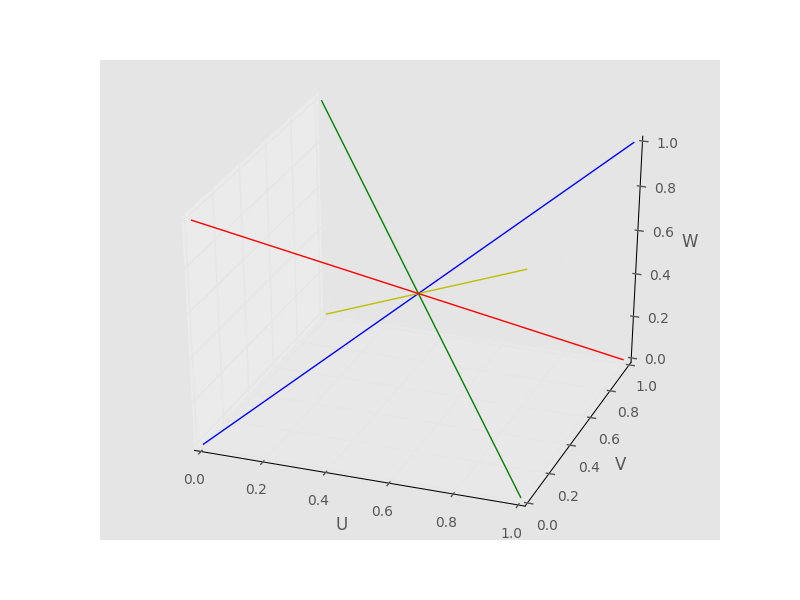
\includegraphics[width=0.7\textwidth]{Diagonals3d.png}
    \caption{Examples of diagonals, \emph{The blue one is [(0,0,0),(1,1,1)], the yellow one is [(0,1,0),(1,0,1)], the green one is [(0,1,1),(1,0,0)],  and the red one is [(0,0,1),(1,1,0)] }}
\end{figure}

\begin{figure}
  
    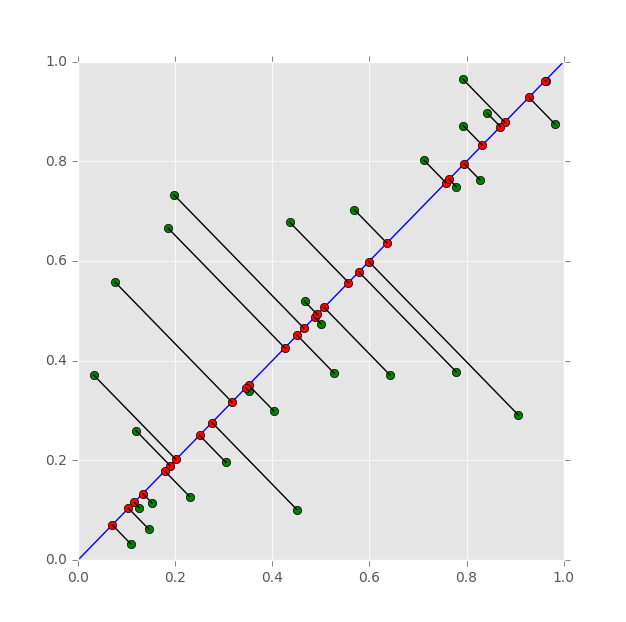
\includegraphics[width=0.7\textwidth]{proj2Ddiag0.png}
    \caption{Projection of 30 points on the [(0,0),(1,1)] diagonal \emph{The diagonal is in blue, the initial points are green and their projections are red.}}
\end{figure}

	\begin{figure}
  
    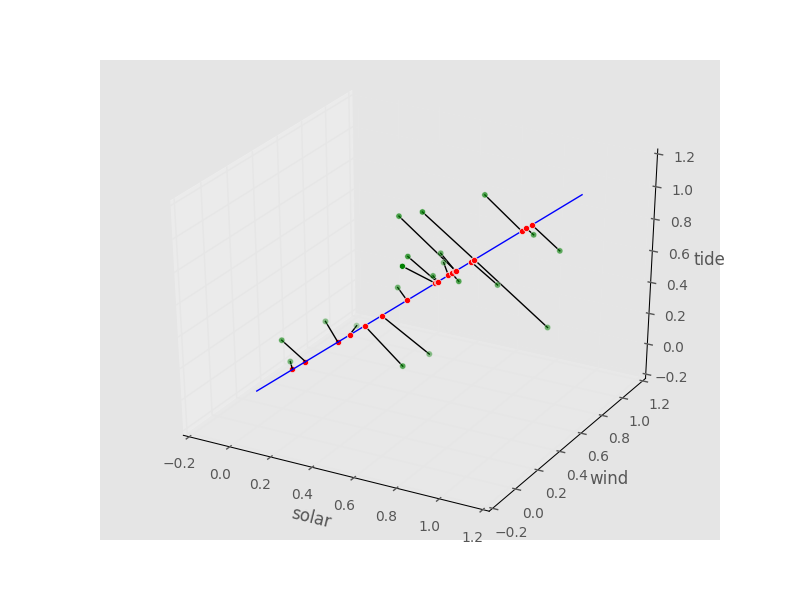
\includegraphics[width=0.7\textwidth]{proj3d.png}
    \caption{Projection of 20 points on the [(0,0,0),(1,1,1)] diagonal \emph{The diagonal is in blue, the initial points are green and their projections are red.}}
\end{figure}
	   
	  \begin{figure}
  
    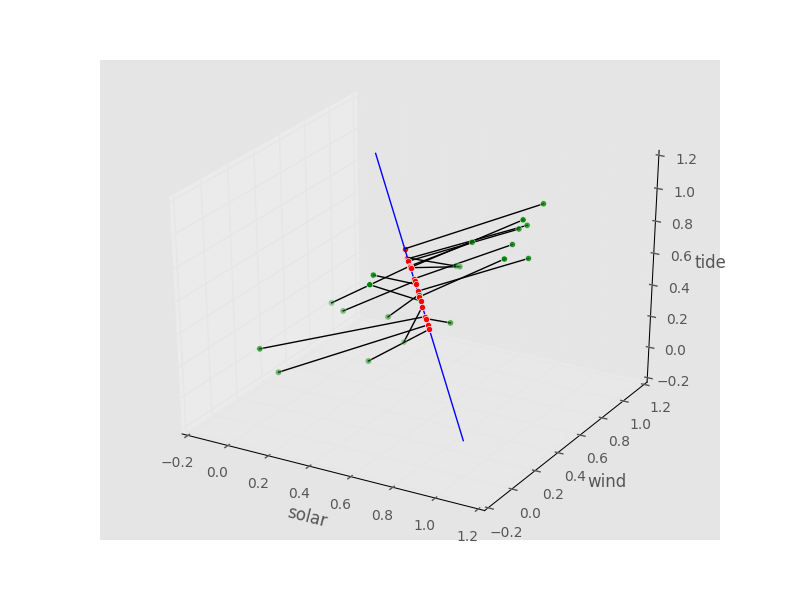
\includegraphics[width=0.7\textwidth]{proj3Ddiag2.png}
    \caption{Projection of 20 points on the [(1,0,0),(0,1,1)] diagonal \emph{The diagonal is in blue, the initial points are green and their projections are red.}}
\end{figure}


	\subsection{Distribution on the diagonal}
	We now want to study the distribution of the points projected on the diagonal to compare it to a uniform distribution. Since the diagonal is a segment, each point x of the diagonal can be described by only one scalar number $\lambda$ : $x = (1-\lambda)a+\lambda b $ (cf Definition of the diagonal). \newline
	$\lambda$ can be understood as the normalised distance between a and x :
	\begin{equation*}
		\| x-a \|	= \| (1-\lambda)a+\lambda b\|
					= \lambda \| a - b \|
					= \lambda \sqrt{d} 
	\end{equation*}
Where $\| . \|$ is a norm in our space.\newline
\newline
But $\lambda$ can be easily evaluated by taking the first coordonates of x : 
	\begin{equation*}
		x_1 = (1-\lambda)a_1 + \lambda b_1 = (1-\lambda) *0 + \lambda *1 = \lambda 
	\end{equation*}
This equality is possible thanks to our useful convention $(a_1,b_1)= (0,1)$.\newline
\newline
We now have a unique number that should be uniformly distributed on [0,1].

	

	  
	  \section{Our algorithm}
	  
	  For each day j do :

\begin{itemize}

\item Thanks to all day \begin{math}i \leq j-1\end{math}, fit a parametric distribution model with copula \begin{math} C_j \end{math}

\item Generate n realizations U of the random variable with the copula dependance and uniform marginals :\newline

	Generate \begin{math} \textbf{U}=(U_1,...,U_n) \end{math} with each \begin{math} U_i = (U_{i,1},...,U_{i,d}) \in [0,1]^d \end{math} \newline
\newline	
	 where \begin{math} \forall i \in \llbracket 1,n \rrbracket , \newline \mathbb{P} (U_{i,1} \leq u_1,..., U_{i,d} \leq u_d )= C(u_1,...,u_d) \text{ and } \newline
	( \forall j \in \llbracket 1,d \rrbracket, U_{i,j} \end{math} is uniformly distributed on [0,1].) \newline
	For example, n=10000  \newline
	
	
	
\item For each diagonal $\Delta$ : 
\item 
Project all the \begin{math} U_i \end{math} on the diagonal
\newline
	Define \begin{math} \textbf{V}_{\Delta} =(V_{\Delta ,1},...,V_{\Delta ,n})=(P_\Delta(U_1),...,P_\Delta(U_n)) \end{math}

\item Define the empirical distribution on this diagonal : \newline
\newline
	\begin{math} F_\Delta (X) = \frac{1}{n} \sum_{k=1}^n \mathds{1}_{X \leq V_{\Delta ,k}} \end{math}
	\newline
	\newline
	where \begin{math} a \leq b \iff \forall i \in \llbracket 1,d \rrbracket,  a_i \leq b_i  \end{math}
	
\item Observe with the data what happened on day j \newline
		Call this observation $O_j = (O_{j,1},...,O_{j,d})$

\item Pass it in the copula space \newline
		Define \begin{math} Q_j = (F_1 (O_{j,1}),...,F_d (O_{j,d})) \end{math} \newline
		where the $F_i$ are the cumulative density functions of the marginals estimated with another method.
		
\item Project $Q_j$ on the diagonal \newline
		Define $R_{\Delta ,j} = P_\Delta (Q_j)$

\item Either define $S_{\Delta,j} = F_\Delta (R_{\Delta,j})  $ \newline
	and compute the distance between the empirical distribution of the $S_{\Delta}=(S_{\Delta,i})_{i \in days}$  and the uniform distribution on [0,1].

\item Or make a rank histogram with the $R_{\Delta}=(R_{\Delta,i})_{i \in days}$
	\begin{math} F_\Delta^{-1} (P_j) \end{math}
	
	\section{Test code}
	
	In this section, I will explain how we computed this algorithm with different parameters. They are arguments of many test functions I wrote and are just strings defining options :\newline
	
	source : the type of power source we want it can be 'solar' or 'wind'\newline
	
	datatype : if the datas is power ('actuals'), errors ('errors), a normal distributed sample ('normal-sample') or a uniformly distributed sample ('uniform-sample'), the two last ones are options to make verifications. \newline
	
	segment_marginals : the way you segment the datas to fit the marginals, you can either take only the date at the hour of your dps ('hour') or fit this marginal with the datas of the whole day ('anytime'). Note : this is not the way the datas are segmented to fit the copula.
	
	kind : which projection you want it can be on a diagonal ('diagonal'), a marginal ('marginal') or can even compose with the kendall function ('kendal'). \newline
	
	index : the index of the diagonal or the marginal you want to project with. Diagonals are indexed in the order of diag. list of diags. Marginals are index as the coordonates. index does not matter for kendall function.\newline
	
	method : way you choose the data to fit the distributions, you can either fit copulas and marginals with the datas of the whole year and check the observation then ('wholeyear'), or you 
	
	
	

\end{itemize}
	
	   
   
   
   
   \begin{thebibliography}{9}

	\bibitem{hamill2000}
  	Thomas M. Hamill,
 	 \emph{Interpretation of Rank Histograms for Verifying Ensemble Forecasts},
  	2000.

	\bibitem{vineconstruction}
  	Kjersti Aas, Claudia Czado, Arnoldo Frigessi, Henrik Bakken,
 	 \emph{Pair-copula construction of multiple dependence},
  	2007.
  	
  	\bibitem{fourcopulas}
  	Kjersti Aas,
 	 \emph{Modeling the dependance structure of financial assets : A survey of four copulas},
  	2004.
  	
  	\bibitem{gaubert}
  	Stéphane Gaubert, Frédéric Bonnans,
  	\emph{Recherche opérationnelle : aspects mathématiques et applications},
  	Editions de l'École polytechnique,
  	2016

	\end{thebibliography}
\end{document}